\documentclass[11pt]{article}
\usepackage[a4paper,margin=1in]{geometry}
\reversemarginpar
\usepackage{mathtools, amsthm, amssymb, amsmath}
\usepackage{multicol}
\usepackage{hyperref}
\usepackage{subcaption}
\usepackage{longtable}
\usepackage{graphicx}
\graphicspath{{./picture/}}
\usepackage{subcaption}
\usepackage{tikz}
\usetikzlibrary{positioning}
\usepackage{rotating}
\usepackage{mfirstuc}

\begin{document}

\begin{figure}
\centering

\begin{subfigure}{\textwidth}
  \centering
  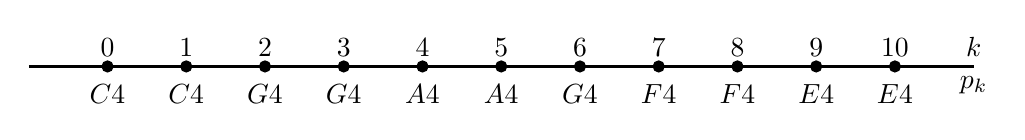
\begin{tikzpicture}
    % Draw number line
    \draw[-, thick] (0,0) -- (12,0) node[below] {$p_k$}  node[above] {$k$};

    % Data
    \foreach \i/\x/\p in {1/C4/0, 2/C4/1, 3/G4/2, 4/G4/3, 5/A4/4, 6/A4/5, 7/G4/6, 8/F4/7, 9/F4/8, 10/E4/9, 11/E4/10} {
      % Draw points and labels
      \filldraw (\i,0) circle (2pt) node[above] {$\p$};
      
      % Draw number scale below the line
      \draw (\i,-0.1) node[below] {$\x$};
    }

  \end{tikzpicture}
  \caption{The first 11 pitches of the Ah vous dirai-je Maman are marked below the 1D axis.}
  \label{subfig2:mp}
\end{subfigure}

\vspace{5pt}

\begin{subfigure}{\textwidth}
  \centering
  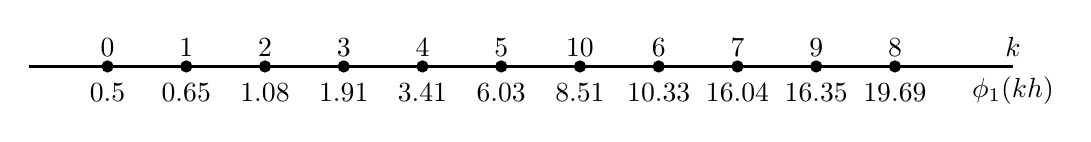
\begin{tikzpicture}
    % Draw number line
    \draw[-, thick] (0,0) -- (12.5,0) node[below] {$\phi_1(kh)$}  node[above] {$k$};

    % Data
    \foreach \i/\x/\p in {1/0.5/0, 2/0.65/1, 3/1.08/2, 4/1.91/3, 5/3.41/4, 6/6.03/5, 7/8.51/10, 8/10.33/6, 9/16.04/7, 10/16.35/9, 11/19.69/8} {
      % Draw points and labels
      \filldraw (\i,0) circle (2pt) node[above] {$\p$};
      
      % Draw number scale below the line
      \draw (\i,-0.1) node[below] {$\x$};
    }

  \end{tikzpicture}
  \caption{The first 11 numerical solution in first component to the Lorenz system with initial condition of $(0.5,0.5,0.5)$ are marked below the 1D axis.}
  \label{subfig2:traj1}
\end{subfigure}

\vspace{5pt}

\begin{subfigure}{\textwidth}
  \centering
  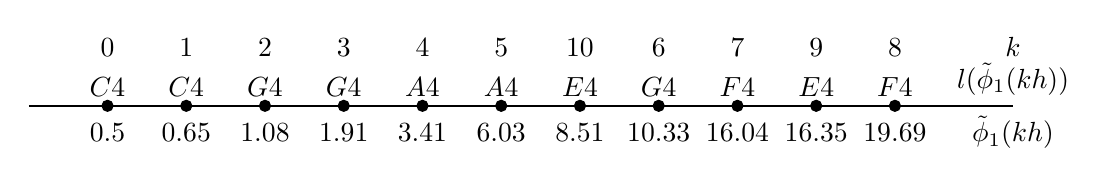
\begin{tikzpicture}
    % Draw number line
    \draw[-, thick] (0,0) -- (12.5,0) node[below] {$\tilde{\phi}_1(kh)$}  node[above] {$l(\tilde{\phi}_1(kh))$} node[above=0.5cm] {$k$};

    % Data
    \foreach \i/\x/\p in {1/0.5/C4, 2/0.65/C4, 3/1.08/G4, 4/1.91/G4, 5/3.41/A4, 6/6.03/A4, 7/8.51/E4, 8/10.33/G4, 9/16.04/F4, 10/16.35/E4, 11/19.69/F4} {
      % Draw points and labels
      \filldraw (\i,0) circle (2pt) node[above] {$\p$};
      
      % Draw number scale below the line
      \draw (\i,-0.1) node[below] {$\x$};
    }
    
    % Display the sequence at each point
    \foreach \i/\x in {1/0, 2/1, 3/2, 4/3, 5/4, 6/5, 7/10, 8/6, 9/7, 10/9, 11/8} {
      \draw (\i,0.5) node[above] {\x};
    }
  \end{tikzpicture}
  \caption{For each component in $\{\phi_1(kh)\}_{k=0}^{10}$, apply the $g(\phi_1(kh))$ mapping.}
  \label{subfig2:traj1mp}

\end{subfigure}

\vspace{5pt}

\begin{subfigure}{\textwidth}
  \centering
  \small{
  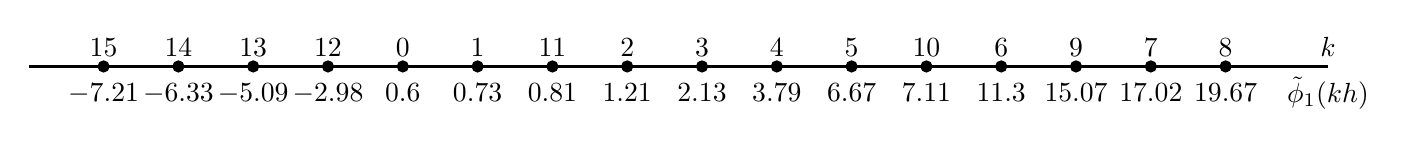
\begin{tikzpicture}
    % Draw number line
    \draw[-, thick] (0,0) -- (16.5,0) node[below] {$\tilde{\phi}_1(kh)$}  node[above] {$k$};

    % Data
    \foreach \i/\x/\p in {1/-7.21/15, 2/-6.33/14, 3/-5.09/13, 4/-2.98/12, 5/0.6/0, 6/0.73/1, 7/0.81/11, 8/1.21/2, 9/2.13/3, 10/3.79/4, 11/6.67/5, 12/7.11/10, 13/11.3/6, 14/15.07/9, 15/17.02/7, 16/19.67/8} {
      % Draw points and labels
      \filldraw (\i*0.95,0) circle (2pt) node[above] {$\p$};
      
      % Draw number scale below the line
      \draw (\i*0.95,-0.1) node[below] {$\x$};
    }

  \end{tikzpicture}}
  \caption{The first 16 numerical solution in first component to the Lorenz system with new initial condition of $(0.6,0.5,0.5)$ are marked below the 1D axis.}
  \label{subfig2:traj2}

\end{subfigure}

\vspace{5pt}

\begin{subfigure}{\textwidth}
  \centering
  \small{
  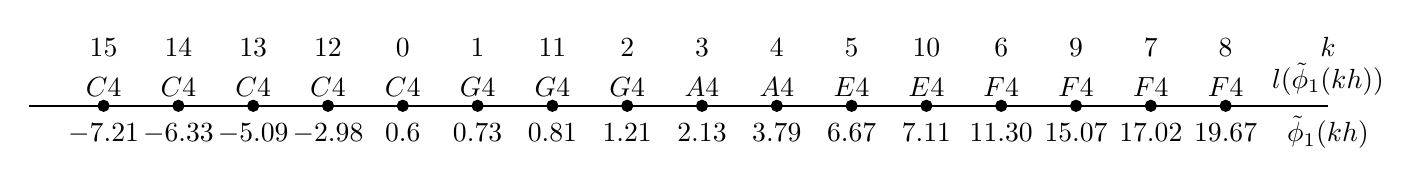
\begin{tikzpicture}
    % Draw number line
    \draw[-, thick] (0,0) -- (16.5,0) node[below] {$\tilde{\phi}_1(kh)$}  node[above] {$l(\tilde{\phi}_1(kh))$} node[above=0.5cm] {$k$};

    % Data
    \foreach \i/\x/\p in {1/-7.21/C4, 2/-6.33/C4, 3/-5.09/C4, 4/-2.98/C4, 5/0.6/C4, 6/0.73/G4, 7/0.81/G4, 8/1.21/G4, 9/2.13/A4, 10/3.79/A4, 11/6.67/E4, 12/7.11/E4, 13/11.30/F4, 14/15.07/F4, 15/17.02/F4, 16/19.67/F4} {
      % Draw points and labels
      \filldraw (\i*0.95,0) circle (2pt) node[above] {$\p$};
      
      % Draw number scale below the line
      \draw (\i*0.95,-0.1) node[below] {$\x$};
    }
    
    % Display the sequence at each point
    \foreach \i/\x in {1/15, 2/14, 3/13, 4/12, 5/0, 6/1, 7/11, 8/2, 9/3, 10/4, 11/5, 12/10, 13/6, 14/9, 15/7, 16/8} {
      \draw (\i*0.95,0.5) node[above] {\x};
    }
  \end{tikzpicture}}
  \caption{For each component in $\{\tilde{\phi}_1(kh)\}_{k=0}^{15}$, apply the $l(\tilde{\phi}_1(kh))$ mapping.}
  \label{subfig2:traj2nmp}

\end{subfigure}

\vspace{5pt}

\begin{subfigure}{\textwidth}
  \centering
  \small{
  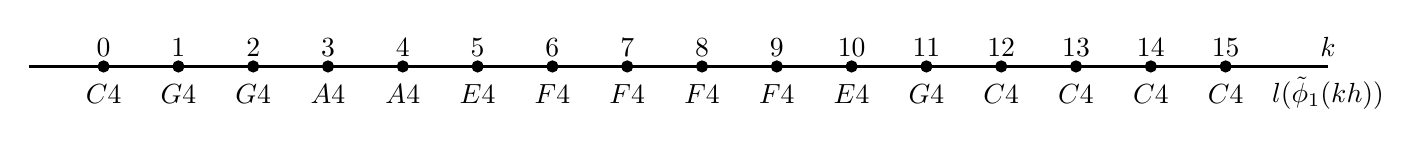
\begin{tikzpicture}
    % Draw number line
    \draw[-, thick] (0,0) -- (16.5,0) node[below] {$l(\tilde{\phi}_1(kh))$}  node[above] {$k$};

    % Data
    \foreach \i/\x/\p in {1/C4/0, 2/G4/1, 3/G4/2, 4/A4/3, 5/A4/4, 6/E4/5, 7/F4/6, 8/F4/7, 9/F4/8, 10/F4/9, 11/E4/10, 12/G4/11, 13/C4/12, 14/C4/13, 15/C4/14, 16/C4/15} {
      % Draw points and labels
      \filldraw (\i*0.95,0) circle (2pt) node[above] {$\p$};
      
      % Draw number scale below the line
      \draw (\i*0.95,-0.1) node[below] {$\x$};
    }

  \end{tikzpicture}}
  \caption{The new variation of the first 16 pitches are marked below the 1D axis.}
  \label{subfig2:nmp}

\end{subfigure}
\end{figure}


\end{document}